\documentclass[11pt]{article}
\usepackage{fullpage,url}
\usepackage{amsmath,amsthm,amssymb}
\usepackage{graphicx}
\usepackage{eso-pic}
\usepackage{bm}
\usepackage{caption}
\usepackage{picins}   
\usepackage{microtype}
\usepackage{subcaption}
\usepackage{url}
\usepackage{enumerate}
\usepackage{pdfpages}
\usepackage{hyperref}
\usepackage[letterpaper,top=1in,bottom=1in,left=1in,right=1in,nohead]{geometry}
\usepackage[export]{adjustbox}

\newcommand{\PhiB}{\mathbf{\Phi}}
\newcommand{\Ll}{\mathcal{L}}
\newcommand{\Nn}{\mathcal{N}}
\newcommand{\Uu}{\mathcal{U}}
\newcommand{\Ee}{\mathcal{E}}
\newcommand{\Aa}{\mathcal{A}}
\newcommand{\Hh}{\mathcal{H}}
\newcommand{\Ii}{\mathcal{I}}
\newcommand{\Vv}{\mathcal{V}}
\newcommand{\Ff}{\mathcal{F}}
\newcommand{\Dd}{\mathcal{D}}
\newcommand{\Tt}{\mathcal{T}}
\newcommand{\Pp}{\mathcal{P}}
\newcommand{\Ss}{\mathcal{S}}
\newcommand{\Cc}{\mathcal{C}}
\newcommand{\Oo}{\mathcal{O}}
\newcommand{\Bb}{\mathcal{B}}
\newcommand{\Rr}{\mathcal{R}}
\newcommand{\Rm}{\mathrm{R}}
\newcommand{\CB}{\mathbf{C}}
\newcommand{\RB}{\mathbf{R}}
\newcommand{\xB}{\mathbf{x}}
\newcommand{\yB}{\mathbf{y}}
\newcommand{\XB}{\mathbf{X}}
\newcommand{\YB}{\mathbf{Y}}
\newcommand{\fB}{\mathbf{f}}
\newcommand{\tB}{\mathbf{t}}
\newcommand{\uB}{\mathbf{u}}
\newcommand{\ZB}{\mathbf{Z}}
\newcommand{\SB}{\mathbf{S}}
\newcommand{\GB}{\mathbf{G}}
\newcommand{\AB}{\mathbf{A}}
\newcommand{\WB}{\mathbf{W}}
\newcommand{\TB}{\mathbf{T}}
\newcommand{\IB}{\mathbf{I}}

\newcommand{\omitme}[1]{}
\newtheorem*{lemma}{Lemma}
\newtheorem{case}{Case}

\makeatletter
\newcommand{\specialnumber}[1]{%
  \def\tagform@##1{\maketag@@@{(\ignorespaces##1\unskip\@@italiccorr#1)}}%
}

\setlength{\parindent}{0in}
\setlength{\parskip}{6pt}

\DeclareMathOperator{\E}{E}
\DeclareMathOperator{\Var}{Var}
\DeclareMathOperator{\Unif}{Unif}

\begin{document}
\thispagestyle{empty}
{\large{\bf CS6320: 3D Computer Vision \hfill Prateep Mukherjee(u0876583)}}\\

{\LARGE{\bf Homework 4}}
\vspace{0.2\baselineskip}
\hrule


{\huge{\bf I. Theoretical Problems}}
    \vspace{-10pt}
    
 \section{Structured Light}   
   \vspace{-10pt}

\subsection{\textbf{2D Triangulation}}
\vspace{-10pt}

\begin{figure*}[!hbt]
\centering
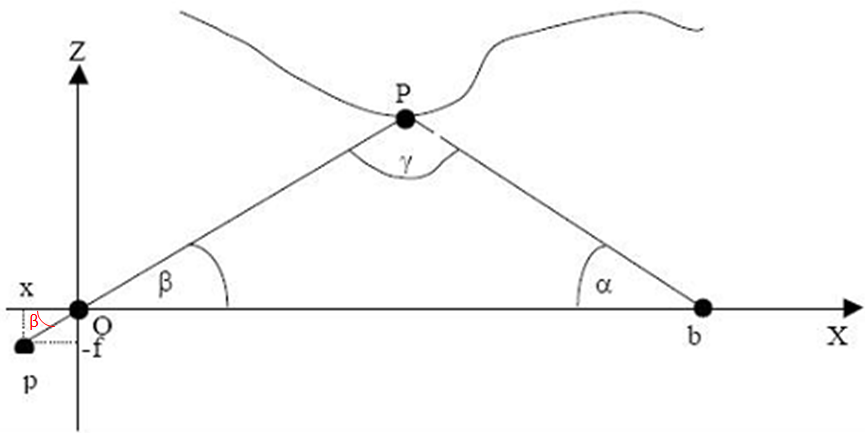
\includegraphics[width=0.5\linewidth]{../im1.png}
\caption{Sketch of 2D Triangulation with angle $\beta$ highlighted in red.}
\label{fig1}
\end{figure*}

Fig. \ref{fig1} shows the sketch for 2D projection. According to similar triangles, we can say $\tan{\beta} = \frac{f}{x}$, implies $\beta = \tan^{-1}(\frac{f}{x})$.

\subsection{\textbf{3D Triangulation}}
\vspace{-10pt}

From the 3D geometry as given in the question(Fig. 2), height of the object $Y_0$ in the world can be expressed in terms of angle $\gamma$ as :
\vspace{-5pt}
$$Y_0 = \frac{b-X_0}{\cos \alpha} \tan \gamma$$ 
Therefore, changing angle $\gamma$ would change the projection point of the laser source on the object, that is change $Y_0$. Thus, changing angle $\gamma$ gives us height of the object which can be used to verify the 3D reconstruction result. 
\section{Motion and Optical Flow}
\vspace{-10pt}

\begin{itemize}
\item Fig \ref{fig2} shows the local vector field for translation of a rectangle within a plane  slanted to the image plane. 

\begin{figure*}[!hbt]
\centering
  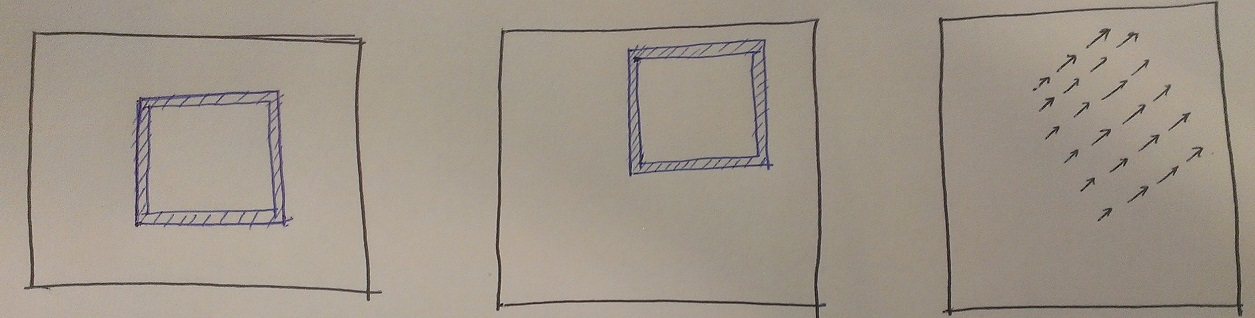
\includegraphics[width=\linewidth]{../rect.jpg}
 \caption{Local displacement field for translation of a rectangle wrt the image plane. {\bf Left, Middle:} two images of the rectangle; {\bf Right:} Displacement vector field.}
 \label{fig2}
\end{figure*}

Fig \ref{fig3} shows the local vector field for rotating of a rectangle within a plane  parallel to the image plane. Arrows show the displacement of the rectangle sides.

\begin{figure*}[!hbt]
\centering
  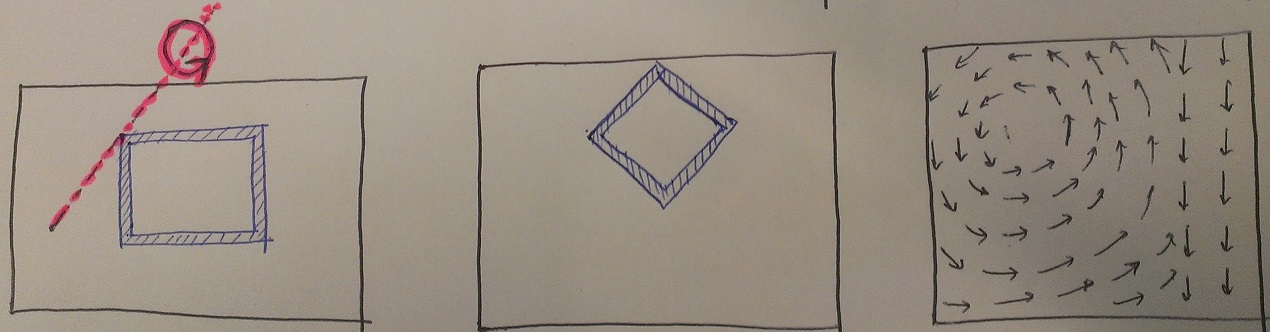
\includegraphics[width=\linewidth]{../rect2.jpg}
 \caption{Local displacement field for rotating  a rectangle parallel to the image plane. {\bf Left, Middle:} two images of the rectangle; {\bf Right:} Displacement vector field. The rotation axis is shown in pink.}
 \label{fig3}
\end{figure*}

\item When we look at the border of the rectangle, the local displacement is seen in the direction in which the rectangle moves. Fig. \ref{fig4} shows the displacement fields for translation and rotation of the rectangle.

\begin{figure*}[!hbt]
\centering
  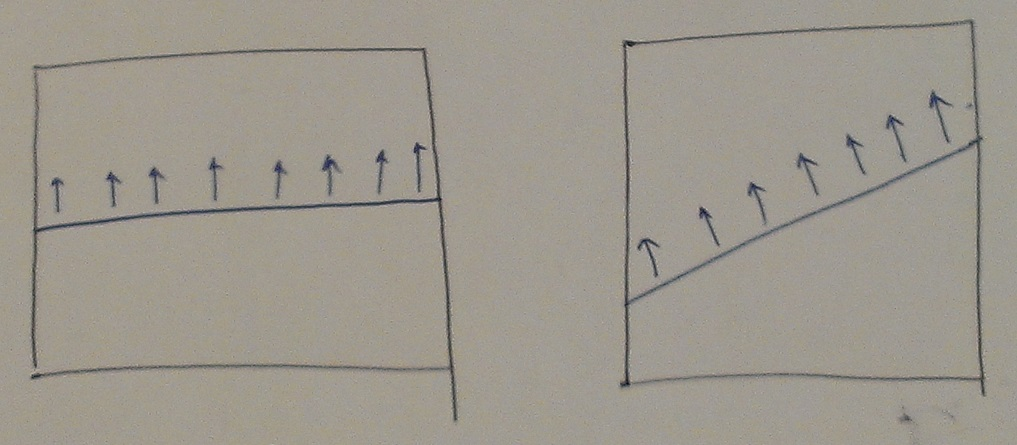
\includegraphics[width=\linewidth]{../IMAG0268.jpg}
 \caption{Local displacement field for rotating  a rectangle parallel to the image plane. {\bf Left, Middle:} two images of the rectangle; {\bf Right:} Displacement vector field. The rotation axis is shown in pink.}
 \label{fig4}
\end{figure*}

\item The true motion of the rectangle can be acquired if there is no aperture problem. The aperture problem occurs when the size of the camera window is too small to get the true velocity vectors. It can be solved by using multiple apertures to capture the image, or if one can see a corner of the square in the aperture.

\item Fig. \ref{fig6} shows the aperture problem with a corner of the square visible. As seen from the picture, it becomes easier to predict the motion of the rectangle if one corner is visible.

\begin{figure*}[!hbt]
\centering
\begin{tabular}{cc  cc}
  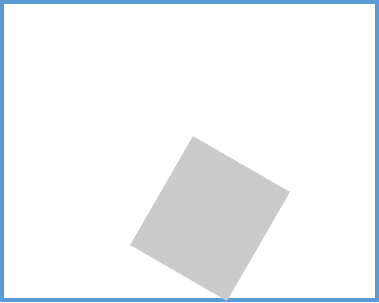
\includegraphics[width=0.4\textwidth]{../ap3.png} &
  
\includegraphics[width=0.4\textwidth]{../ap4.png} \\
  (a) & (b) \\
  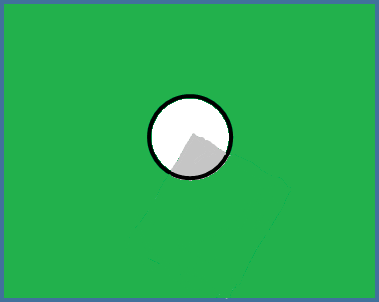
\includegraphics[width=0.4\textwidth]{../ap1.png} &
  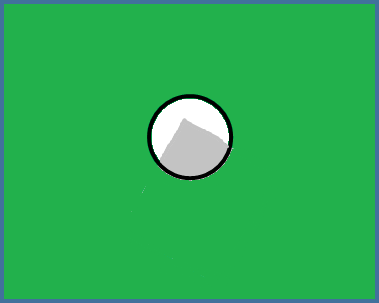
\includegraphics[width=0.4\textwidth]{../ap2.png} \\
  (c) & (d)
 \end{tabular}
 \vspace{-10pt}
 \caption{{\bf (a,b)} Two images show translation of a rectangle;  {\bf (c,d)} Motion of the square as seen through an aperture.}
 \label{fig6}
\end{figure*}
\end{itemize}

%\clearpage

{\huge{\bf II. Practical Problems}}

\begin{figure*}[!hbt]
\centering
\begin{tabular}{cc}
  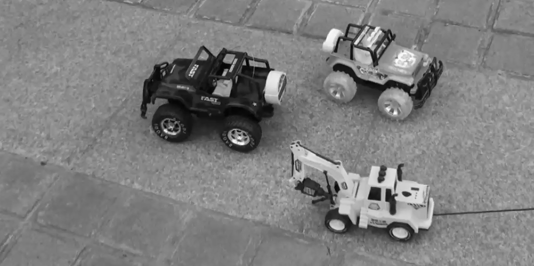
\includegraphics[width=0.5\textwidth]{../toy-car-images-bw/toy_formatted2.png} &
  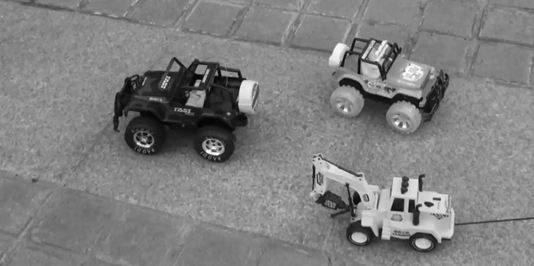
\includegraphics[width=0.5\textwidth]{../toy-car-images-bw/toy_formatted9.png} \\
  (a) & (b) \\
  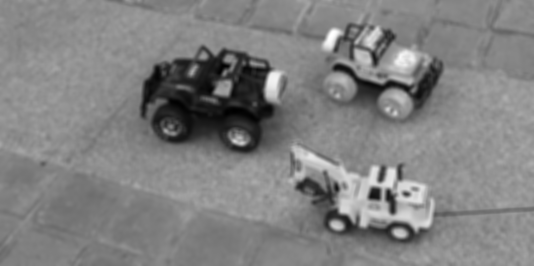
\includegraphics[width=0.5\textwidth]{../im2_smooth.png} &
    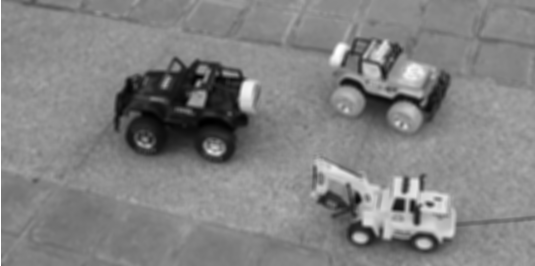
\includegraphics[width=0.5\textwidth]{../im9_smooth.png} \\
  (c) & (d) \\
  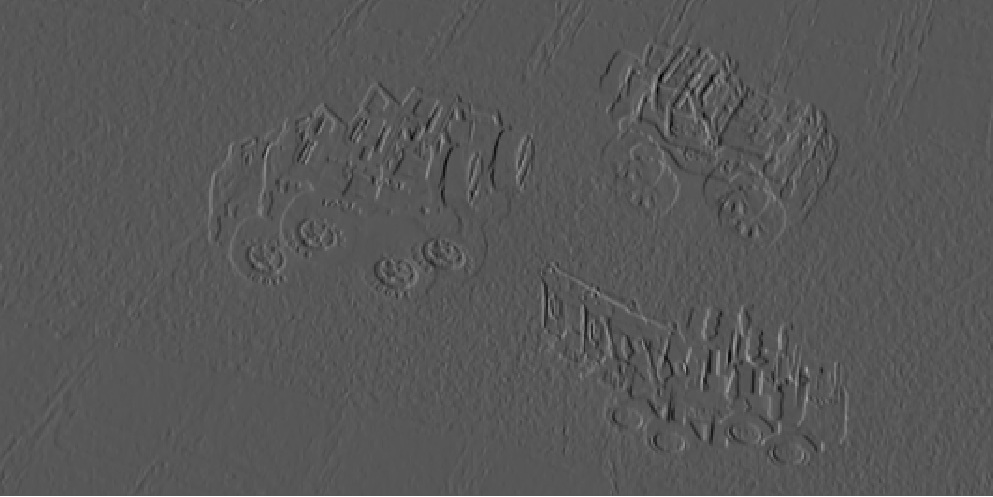
\includegraphics[width=0.5\textwidth]{../Ex2-9.png} &
  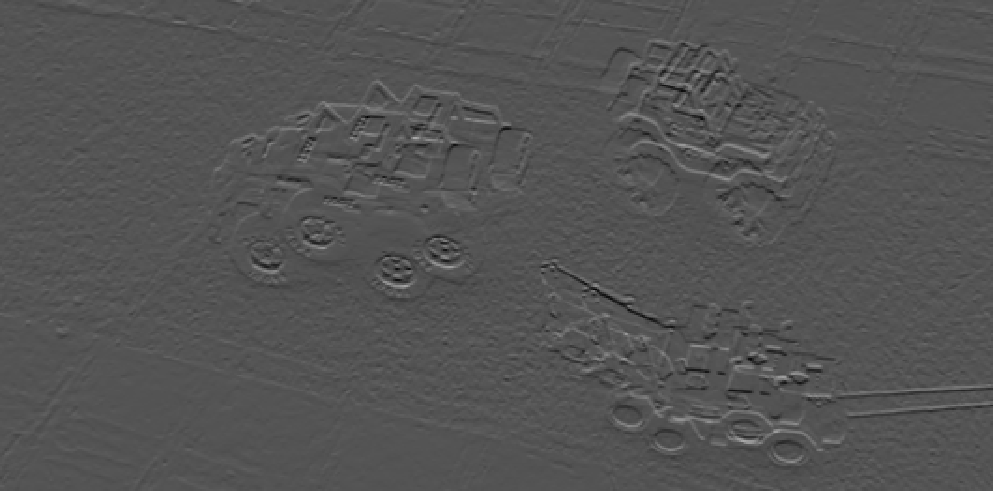
\includegraphics[width=0.5\textwidth]{../Ey2-9.png} \\
  (e) & (f)  \\
  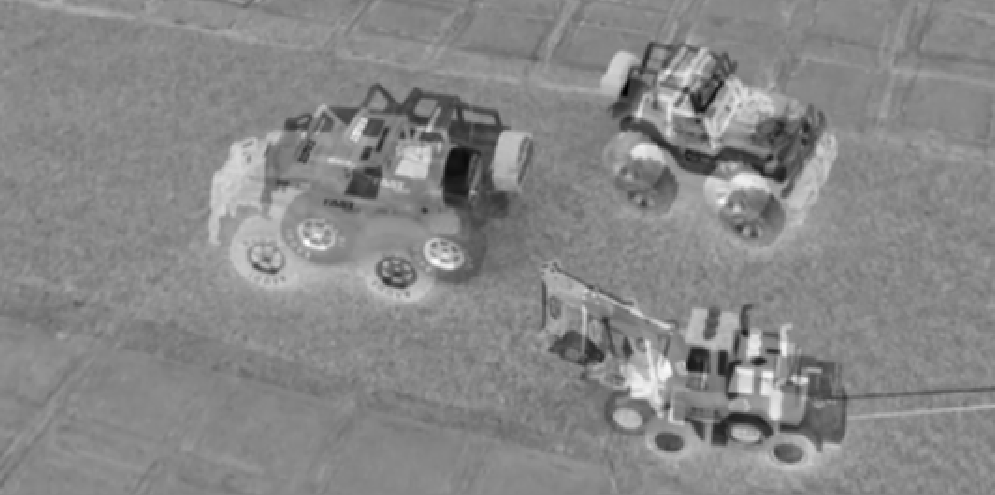
\includegraphics[width=0.5\textwidth]{../Et2-9.png} &
  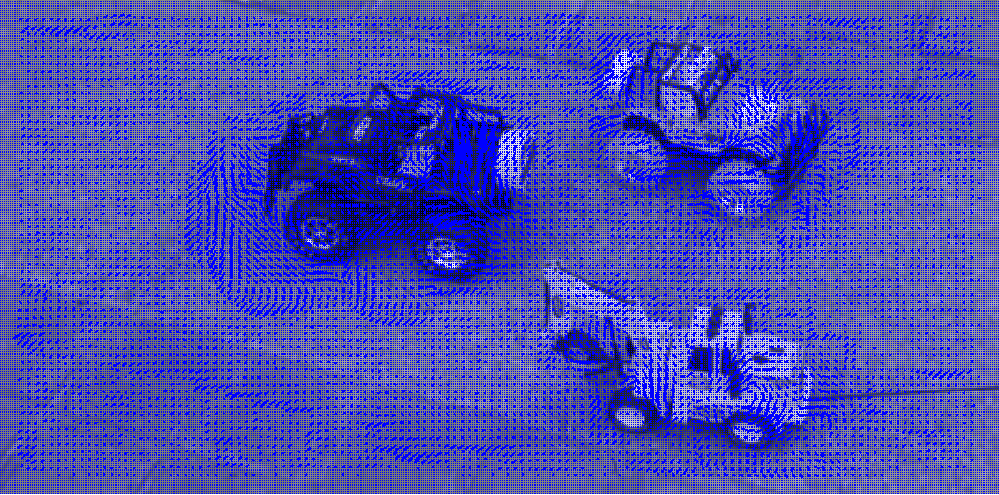
\includegraphics[width=0.5\textwidth]{../car2-9_lk.png} \\
  (g) & (h) \\
 \end{tabular}
 \vspace{-10pt}
 \caption{ Experiment showing the different stages of the standard optical flow algorithm. {\bf (a,b)} toy2.png and toy3.png, images captured from a video sequence; {\bf (c,d)} blurred versions of the above images; {\bf (e,f)} Gradients in x and y directions, that is, $\frac{\partial I}{\partial x}$ and $\frac{\partial I}{\partial y}$; {\bf (g)} The temporal difference, $I_t = $ toy2.png $-$ toy3.png; {\bf (h)} Flow vectors($u,v$) overlayed on toy2.png.}
 \label{fig7}
\end{figure*}

\begin{figure*}[!hbt]
\centering
\begin{tabular}{cc}
  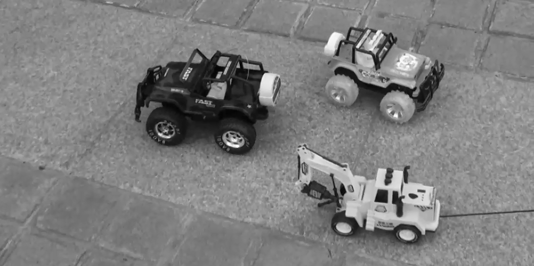
\includegraphics[width=0.5\textwidth]{../toy-car-images-bw/toy_formatted4.png} &
  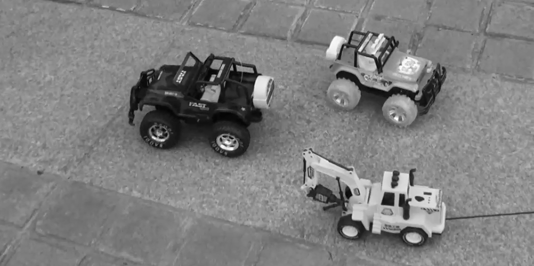
\includegraphics[width=0.5\textwidth]{../toy-car-images-bw/toy_formatted5.png} \\
  (a) & (b) \\
  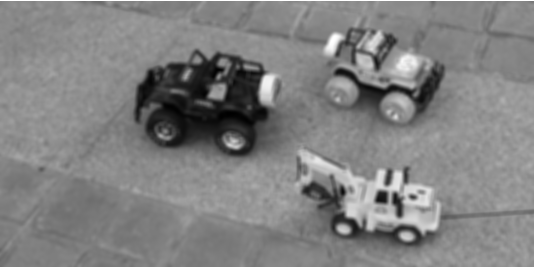
\includegraphics[width=0.5\textwidth]{../im4_smooth.png} &
    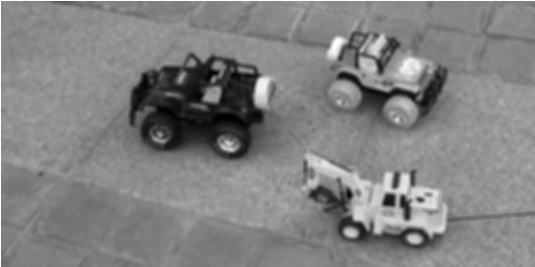
\includegraphics[width=0.5\textwidth]{../im5_smooth.png} \\
  (c) & (d) \\
  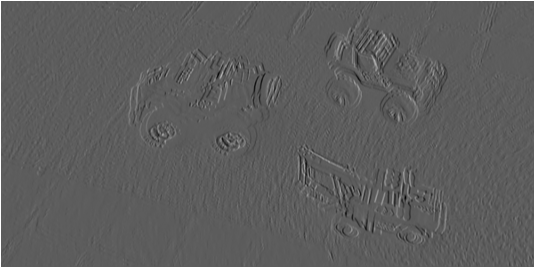
\includegraphics[width=0.5\textwidth]{../Ex4-5.png} &
  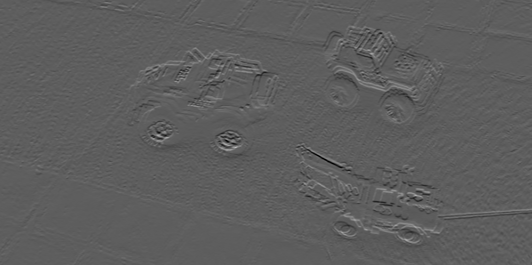
\includegraphics[width=0.5\textwidth]{../Ey4-5.png} \\
  (e) & (f)  \\
  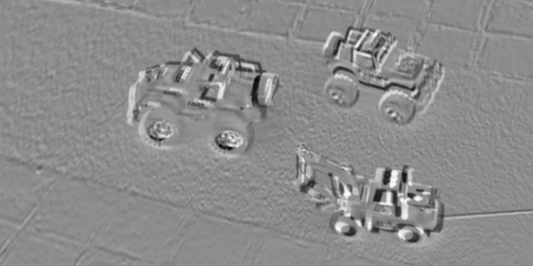
\includegraphics[width=0.5\textwidth]{../Et4-5.png} &
  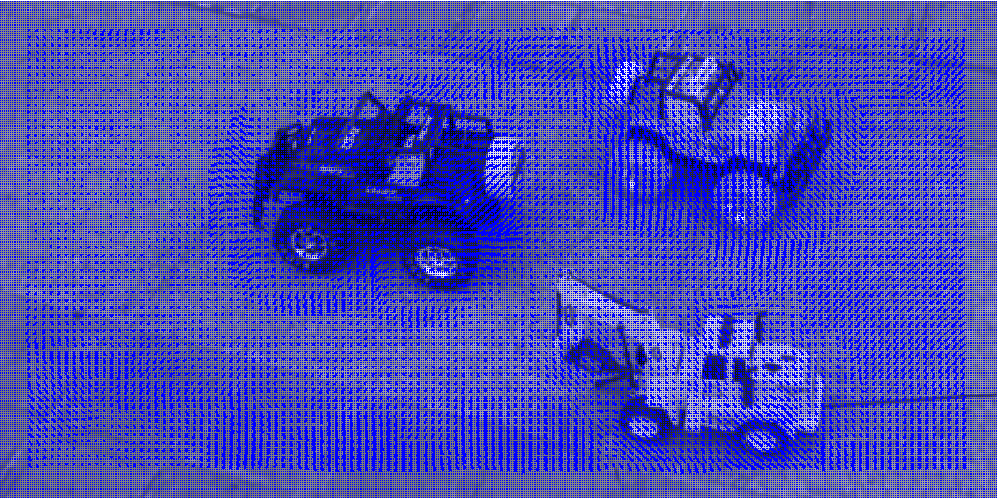
\includegraphics[width=0.5\textwidth]{../car4-5_lk.png} \\
  (g) & (h) \\
 \end{tabular}
 \vspace{-10pt}
 \caption{ Another experiment with different set of consecutive images. {\bf (a,b)} toy4.png and toy5.png, consecutive images captured from a video sequence; {\bf (c,d)} blurred versions of the above images; {\bf (e,f)} Gradients in x and y directions, that is, $\frac{\partial I}{\partial x}$ and $\frac{\partial I}{\partial y}$; {\bf (g)} The temporal difference, $I_t = $ toy4.png $-$ toy5.png; {\bf (h)} Flow vectors($u,v$) overlayed on toy4.png.}
 \label{fig8}
\end{figure*}

Figs. (\ref{fig7} , \ref{fig8}) shows two experiments with the optical flow method. In each experiment, I choose 2 consecutive frames from a video sequence and try to predict the motion of objects. The standard optical flow objective looks as follows:
\vspace{-5pt}
$$ I_x u + I_y v = - I_t$$ 

where $I_x$ and $I_y$ are the spatial derivatives in horizontal and vertical directions, $u,v$ are the velocity components horizontal and vertical, and $I_t$ is the temporal gradient($I_t = I(x,y,t+1) - I(x,y,t)$). These components of the optical flow algorithm are shown in Fig. (\ref{fig7} , \ref{fig8}) in order : $I_x$({\bf \ref{fig7}e, \ref{fig8}e}), $I_y$({\bf \ref{fig7}f, \ref{fig8}f}), $I_t$({\bf \ref{fig7}g, \ref{fig8}g}). The last figure in each experiment shows the velocity vector field computed using optical flow. In both cases(\ref{fig7}h, \ref{fig8}h), considerable motion is seen near the cars, which are actually the objects in motion in the video sequence.

Next, I test the standard patch-based method with Horn-Schunck's regularized method. The result is shown in Fig. \ref{fig9}. Qualitatively, the two methods acquire the motion field well for objects which have small motion. For example, Fig. \ref{fig9}(a,b) shows the flow field for two consecutive frames. The maximum flow obtained for the two methods are: {\bf 0.8676(Horn-Schunck)} and {\bf 0.8408(Patch-based)}. Fig. \ref{fig9}(c,d) shows the flow field for two extremes(toy2.png and toy9.png) which have considerable motion. The maximum flow obtained were: {\bf 0.6371 (Horn-Schunck)} and {\bf 8.5371(Patch-based)}. Thus, for considerable motion, the patch-based method seems to work better against regularized. This conclusion is based on the fact that the images considered show considerable motion of the foreground objects, and a small flow does not justify that motion. However, in order to fairly judge the methods, we would need the ground-truth values of velocities for the objects.
\vspace{-10pt}
\begin{figure*}[!hbt]
\begin{tabular}{cccc}
\hspace{-30pt}
  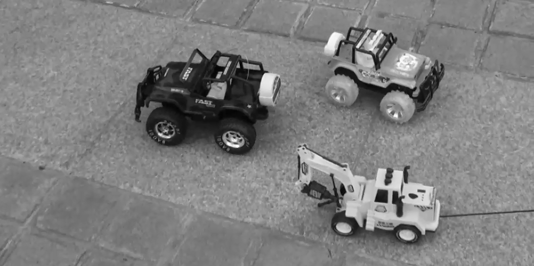
\includegraphics[width=0.25\linewidth]{../toy-car-images-bw/toy_formatted4.png} &  
  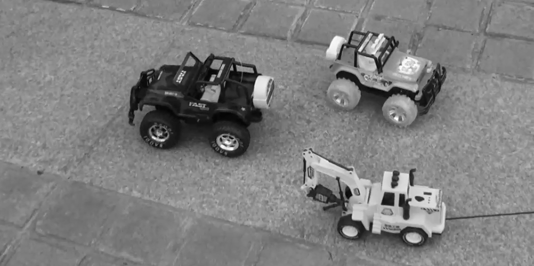
\includegraphics[width=0.25\linewidth]{../toy-car-images-bw/toy_formatted5.png} &
  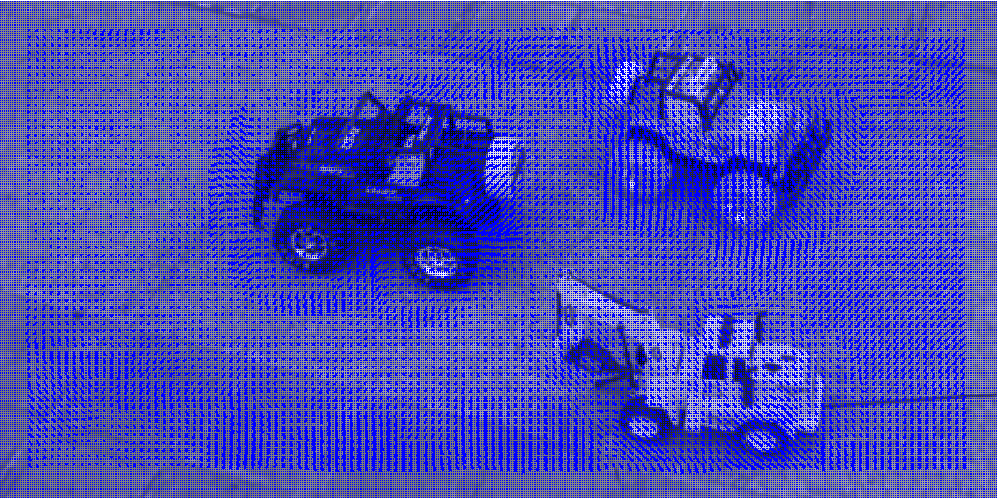
\includegraphics[width=0.25\linewidth]{../car4-5_lk.png} &
  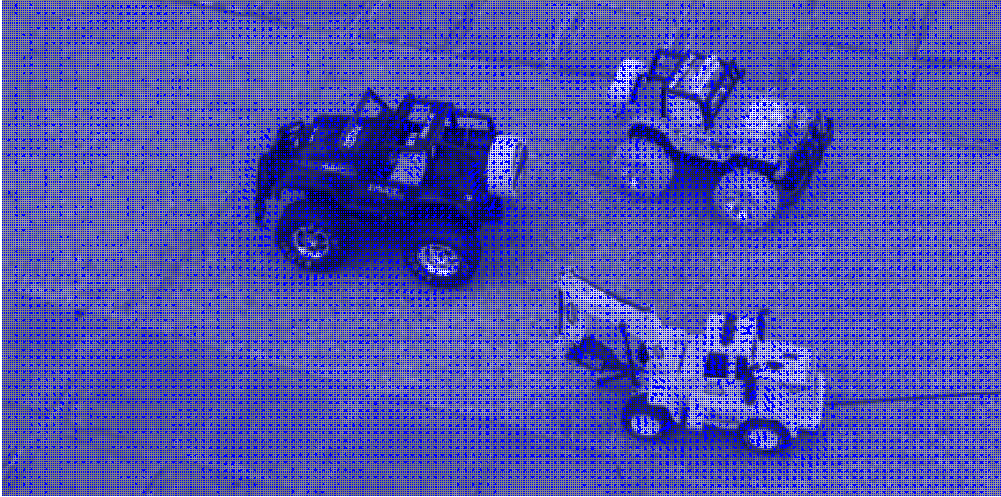
\includegraphics[width=0.25\linewidth]{../car4-5_hs.png} \\
  (a) & (b) & (c) & (d)\\
  \hspace{-30pt}
  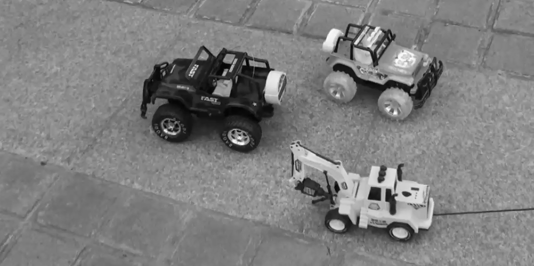
\includegraphics[width=0.25\linewidth]{../toy-car-images-bw/toy_formatted2.png} &
  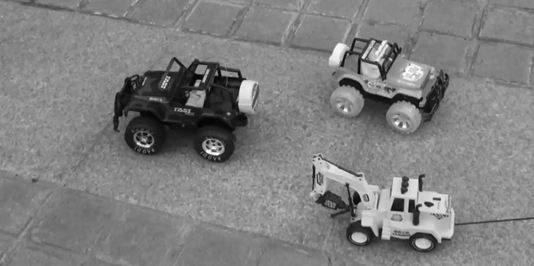
\includegraphics[width=0.25\linewidth]{../toy-car-images-bw/toy_formatted9.png} &
  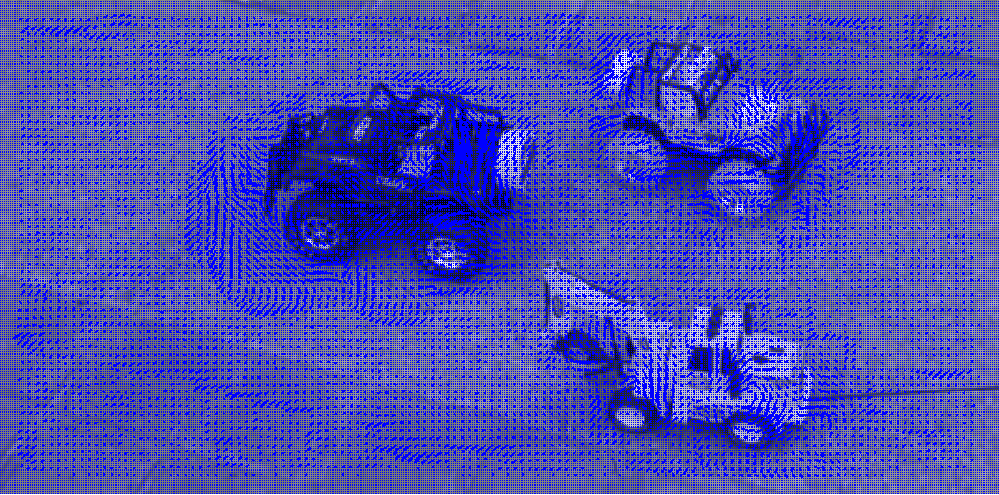
\includegraphics[width=0.25\linewidth]{../car2-9_lk.png} &
  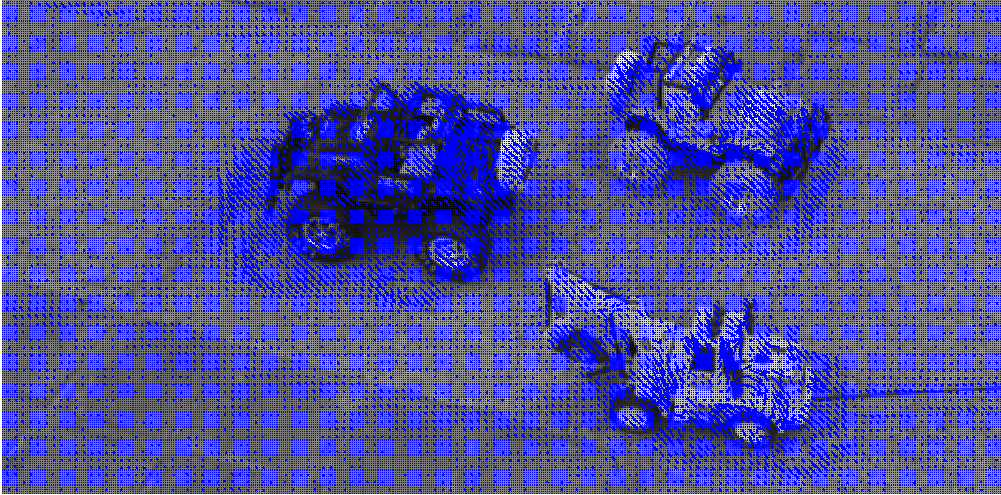
\includegraphics[width=0.25\linewidth]{../car2-9_hs.png} \\
  (e) & (f) & (g) & (h)\\
 \end{tabular}
 \vspace{-10pt}
 \caption{{\bf (a,b,e,f)} toy2.png, toy9.png, toy4.png, toy5.png; {\bf (c,g)} Optical flow field obtained using $2\times2$ patch based neighborhood; {\bf (d,h)} Flow vector field computed using Horn-Schunck regularized method. Top row is computed for pair(toy4.png, toy5.png), Bottom row for (toy2.png, toy9.png).}
 \label{fig9}
\end{figure*}
\vspace{-25pt}
\begin{figure*}[hb]
\begin{tabular}{ccc}
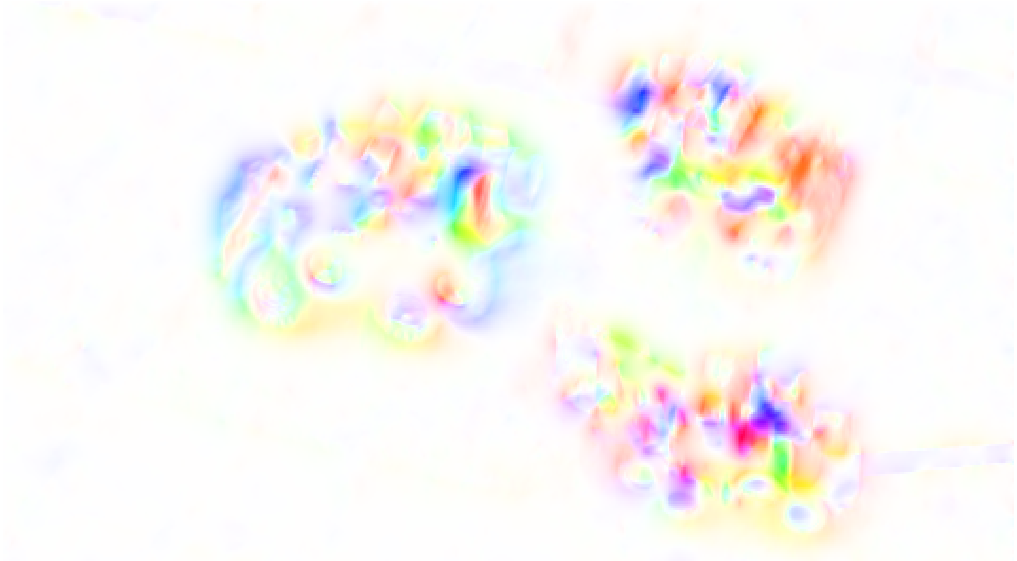
\includegraphics[width=0.5\linewidth]{../img_hs.png} &
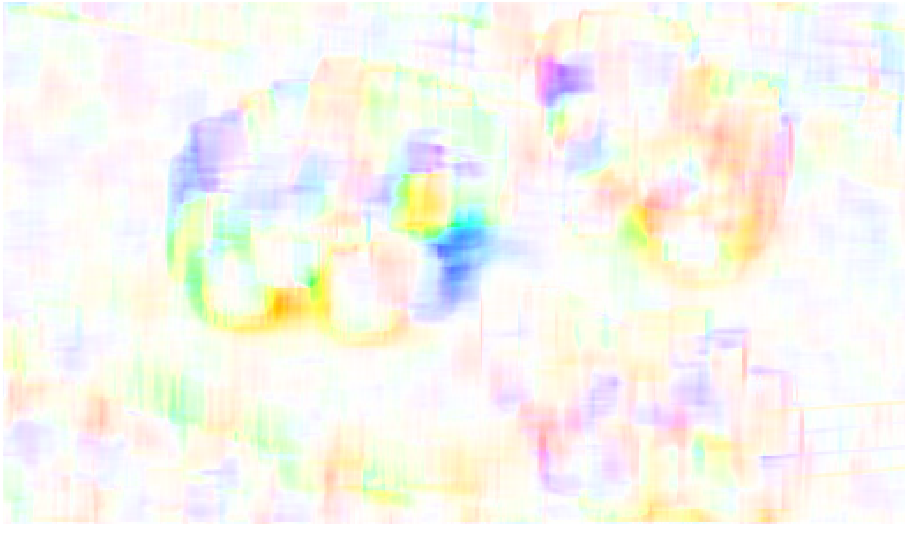
\includegraphics[width=0.47\linewidth]{../img_lk.png} &
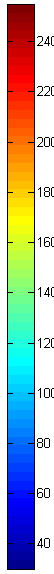
\includegraphics[width=0.03\linewidth,height=4.5cm]{../colorbar.png} \\
\end{tabular}
\caption{Color images of the flow vector field shown using a colorwheel generated from \url{http://members.shaw.ca/quadibloc/other/colint.htm}. {\bf Left:} Patch-based, {\bf Right:} Horn-Schunck}
\label{fig10}
\end{figure*}


\end{document}